% Created by tikzDevice version 0.10.1 on 2020-02-15 15:55:10
% !TEX encoding = UTF-8 Unicode
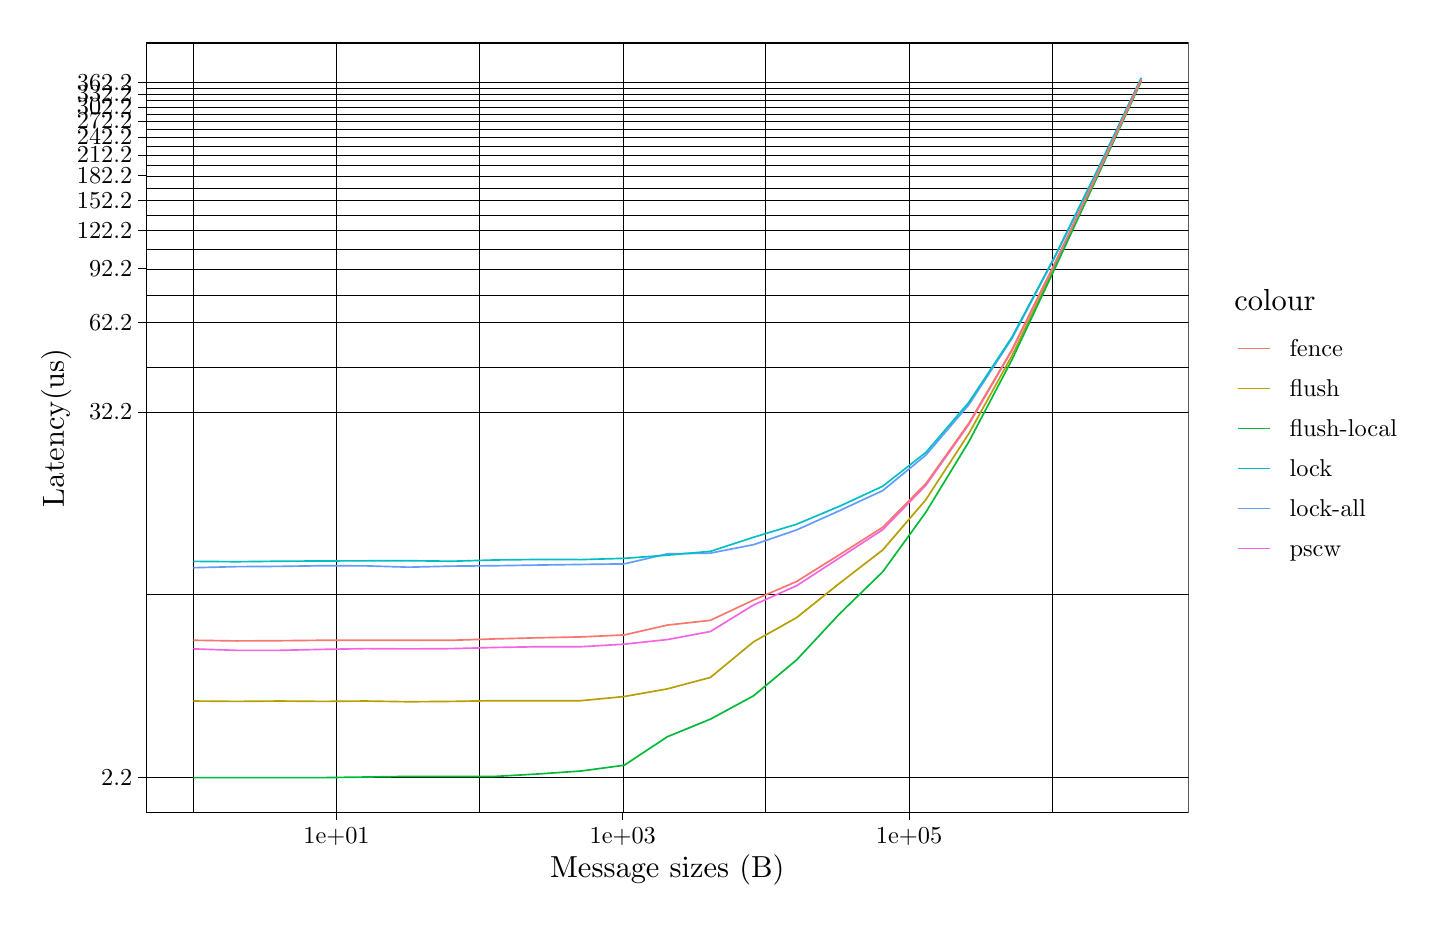
\begin{tikzpicture}[x=1pt,y=1pt]
\definecolor{fillColor}{RGB}{255,255,255}
\path[use as bounding box,fill=fillColor,fill opacity=0.00] (0,0) rectangle (505.89,314.37);
\begin{scope}
\path[clip] (  0.00,  0.00) rectangle (505.89,314.37);
\definecolor{drawColor}{RGB}{255,255,255}
\definecolor{fillColor}{RGB}{255,255,255}

\path[draw=drawColor,line width= 0.6pt,line join=round,line cap=round,fill=fillColor] (  0.00,  0.00) rectangle (505.89,314.37);
\end{scope}
\begin{scope}
\path[clip] ( 42.76, 30.72) rectangle (419.53,308.87);
\definecolor{fillColor}{RGB}{255,255,255}

\path[fill=fillColor] ( 42.76, 30.72) rectangle (419.53,308.87);
\definecolor{drawColor}{RGB}{0,0,0}

\path[draw=drawColor,line width= 0.0pt,line join=round] ( 42.76,109.43) --
	(419.53,109.43);

\path[draw=drawColor,line width= 0.0pt,line join=round] ( 42.76,191.70) --
	(419.53,191.70);

\path[draw=drawColor,line width= 0.0pt,line join=round] ( 42.76,217.60) --
	(419.53,217.60);

\path[draw=drawColor,line width= 0.0pt,line join=round] ( 42.76,234.22) --
	(419.53,234.22);

\path[draw=drawColor,line width= 0.0pt,line join=round] ( 42.76,246.56) --
	(419.53,246.56);

\path[draw=drawColor,line width= 0.0pt,line join=round] ( 42.76,256.39) --
	(419.53,256.39);

\path[draw=drawColor,line width= 0.0pt,line join=round] ( 42.76,264.57) --
	(419.53,264.57);

\path[draw=drawColor,line width= 0.0pt,line join=round] ( 42.76,271.58) --
	(419.53,271.58);

\path[draw=drawColor,line width= 0.0pt,line join=round] ( 42.76,277.71) --
	(419.53,277.71);

\path[draw=drawColor,line width= 0.0pt,line join=round] ( 42.76,283.16) --
	(419.53,283.16);

\path[draw=drawColor,line width= 0.0pt,line join=round] ( 42.76,288.06) --
	(419.53,288.06);

\path[draw=drawColor,line width= 0.0pt,line join=round] ( 42.76,292.52) --
	(419.53,292.52);

\path[draw=drawColor,line width= 0.0pt,line join=round] ( 59.89, 30.72) --
	( 59.89,308.87);

\path[draw=drawColor,line width= 0.0pt,line join=round] (163.32, 30.72) --
	(163.32,308.87);

\path[draw=drawColor,line width= 0.0pt,line join=round] (266.76, 30.72) --
	(266.76,308.87);

\path[draw=drawColor,line width= 0.0pt,line join=round] (370.20, 30.72) --
	(370.20,308.87);

\path[draw=drawColor,line width= 0.1pt,line join=round] ( 42.76, 43.37) --
	(419.53, 43.37);

\path[draw=drawColor,line width= 0.1pt,line join=round] ( 42.76,175.49) --
	(419.53,175.49);

\path[draw=drawColor,line width= 0.1pt,line join=round] ( 42.76,207.91) --
	(419.53,207.91);

\path[draw=drawColor,line width= 0.1pt,line join=round] ( 42.76,227.29) --
	(419.53,227.29);

\path[draw=drawColor,line width= 0.1pt,line join=round] ( 42.76,241.16) --
	(419.53,241.16);

\path[draw=drawColor,line width= 0.1pt,line join=round] ( 42.76,251.96) --
	(419.53,251.96);

\path[draw=drawColor,line width= 0.1pt,line join=round] ( 42.76,260.82) --
	(419.53,260.82);

\path[draw=drawColor,line width= 0.1pt,line join=round] ( 42.76,268.33) --
	(419.53,268.33);

\path[draw=drawColor,line width= 0.1pt,line join=round] ( 42.76,274.84) --
	(419.53,274.84);

\path[draw=drawColor,line width= 0.1pt,line join=round] ( 42.76,280.59) --
	(419.53,280.59);

\path[draw=drawColor,line width= 0.1pt,line join=round] ( 42.76,285.73) --
	(419.53,285.73);

\path[draw=drawColor,line width= 0.1pt,line join=round] ( 42.76,290.39) --
	(419.53,290.39);

\path[draw=drawColor,line width= 0.1pt,line join=round] ( 42.76,294.65) --
	(419.53,294.65);

\path[draw=drawColor,line width= 0.1pt,line join=round] (111.60, 30.72) --
	(111.60,308.87);

\path[draw=drawColor,line width= 0.1pt,line join=round] (215.04, 30.72) --
	(215.04,308.87);

\path[draw=drawColor,line width= 0.1pt,line join=round] (318.48, 30.72) --
	(318.48,308.87);
\definecolor{drawColor}{RGB}{97,156,255}

\path[draw=drawColor,line width= 0.6pt,line join=round] ( 59.89,119.23) --
	( 75.45,119.61) --
	( 91.02,119.71) --
	(106.59,119.94) --
	(122.16,119.89) --
	(137.73,119.42) --
	(153.30,119.80) --
	(168.87,119.94) --
	(184.44,120.18) --
	(200.01,120.41) --
	(215.58,120.60) --
	(231.14,124.24) --
	(246.71,124.50) --
	(262.28,127.55) --
	(277.85,132.87) --
	(293.42,139.87) --
	(308.99,147.10) --
	(324.56,159.92) --
	(340.13,178.18) --
	(355.70,202.12) --
	(371.27,231.66) --
	(386.83,263.34) --
	(402.40,296.19);
\definecolor{drawColor}{RGB}{0,191,196}

\path[draw=drawColor,line width= 0.6pt,line join=round] ( 59.89,121.52) --
	( 75.45,121.39) --
	( 91.02,121.57) --
	(106.59,121.66) --
	(122.16,121.71) --
	(137.73,121.75) --
	(153.30,121.57) --
	(168.87,122.02) --
	(184.44,122.20) --
	(200.01,122.16) --
	(215.58,122.61) --
	(231.14,123.76) --
	(246.71,125.14) --
	(262.28,130.22) --
	(277.85,134.94) --
	(293.42,141.46) --
	(308.99,148.68) --
	(324.56,160.88) --
	(340.13,179.04) --
	(355.70,202.60) --
	(371.27,231.94) --
	(386.83,263.46) --
	(402.40,296.23);
\definecolor{drawColor}{RGB}{183,159,0}

\path[draw=drawColor,line width= 0.6pt,line join=round] ( 59.89, 71.05) --
	( 75.45, 70.92) --
	( 91.02, 71.05) --
	(106.59, 70.92) --
	(122.16, 71.05) --
	(137.73, 70.79) --
	(153.30, 70.92) --
	(168.87, 71.18) --
	(184.44, 71.18) --
	(200.01, 71.18) --
	(215.58, 72.68) --
	(231.14, 75.44) --
	(246.71, 79.58) --
	(262.28, 92.44) --
	(277.85,101.19) --
	(293.42,113.65) --
	(308.99,125.65) --
	(324.56,143.81) --
	(340.13,167.76) --
	(355.70,195.90) --
	(371.27,228.35) --
	(386.83,261.58) --
	(402.40,295.26);
\definecolor{drawColor}{RGB}{0,186,56}

\path[draw=drawColor,line width= 0.6pt,line join=round] ( 59.89, 43.37) --
	( 75.45, 43.37) --
	( 91.02, 43.37) --
	(106.59, 43.37) --
	(122.16, 43.59) --
	(137.73, 43.81) --
	(153.30, 43.81) --
	(168.87, 43.81) --
	(184.44, 44.69) --
	(200.01, 45.77) --
	(215.58, 47.86) --
	(231.14, 58.14) --
	(246.71, 64.51) --
	(262.28, 72.93) --
	(277.85, 85.91) --
	(293.42,102.62) --
	(308.99,117.77) --
	(324.56,139.27) --
	(340.13,164.81) --
	(355.70,194.44) --
	(371.27,227.57) --
	(386.83,261.20) --
	(402.40,295.07);
\definecolor{drawColor}{RGB}{245,100,227}

\path[draw=drawColor,line width= 0.6pt,line join=round] ( 59.89, 89.89) --
	( 75.45, 89.37) --
	( 91.02, 89.37) --
	(106.59, 89.72) --
	(122.16, 89.98) --
	(137.73, 89.89) --
	(153.30, 89.98) --
	(168.87, 90.41) --
	(184.44, 90.67) --
	(200.01, 90.67) --
	(215.58, 91.60) --
	(231.14, 93.26) --
	(246.71, 96.17) --
	(262.28,105.75) --
	(277.85,112.73) --
	(293.42,122.83) --
	(308.99,132.98) --
	(324.56,149.00) --
	(340.13,171.06) --
	(355.70,197.81) --
	(371.27,229.37) --
	(386.83,262.16) --
	(402.40,295.55);
\definecolor{drawColor}{RGB}{248,118,109}

\path[draw=drawColor,line width= 0.6pt,line join=round] ( 59.89, 93.01) --
	( 75.45, 92.77) --
	( 91.02, 92.85) --
	(106.59, 93.01) --
	(122.16, 93.01) --
	(137.73, 93.01) --
	(153.30, 93.01) --
	(168.87, 93.50) --
	(184.44, 93.90) --
	(200.01, 94.22) --
	(215.58, 94.93) --
	(231.14, 98.49) --
	(246.71,100.21) --
	(262.28,107.54) --
	(277.85,114.24) --
	(293.42,123.98) --
	(308.99,133.85) --
	(324.56,149.60) --
	(340.13,171.50) --
	(355.70,198.06) --
	(371.27,229.49) --
	(386.83,262.18) --
	(402.40,295.58);
\definecolor{drawColor}{RGB}{0,0,0}

\path[draw=drawColor,line width= 0.6pt,line join=round,line cap=round] ( 42.76, 30.72) rectangle (419.53,308.87);
\end{scope}
\begin{scope}
\path[clip] (  0.00,  0.00) rectangle (505.89,314.37);
\definecolor{drawColor}{RGB}{0,0,0}

\node[text=drawColor,anchor=base west,inner sep=0pt, outer sep=0pt, scale=  0.88] at ( 26.57, 40.55) {2.2};

\node[text=drawColor,anchor=base west,inner sep=0pt, outer sep=0pt, scale=  0.88] at ( 22.17,172.67) {32.2};

\node[text=drawColor,anchor=base west,inner sep=0pt, outer sep=0pt, scale=  0.88] at ( 22.17,205.08) {62.2};

\node[text=drawColor,anchor=base west,inner sep=0pt, outer sep=0pt, scale=  0.88] at ( 22.17,224.46) {92.2};

\node[text=drawColor,anchor=base west,inner sep=0pt, outer sep=0pt, scale=  0.88] at ( 17.77,238.33) {122.2};

\node[text=drawColor,anchor=base west,inner sep=0pt, outer sep=0pt, scale=  0.88] at ( 17.77,249.14) {152.2};

\node[text=drawColor,anchor=base west,inner sep=0pt, outer sep=0pt, scale=  0.88] at ( 17.77,258.00) {182.2};

\node[text=drawColor,anchor=base west,inner sep=0pt, outer sep=0pt, scale=  0.88] at ( 17.77,265.50) {212.2};

\node[text=drawColor,anchor=base west,inner sep=0pt, outer sep=0pt, scale=  0.88] at ( 17.77,272.02) {242.2};

\node[text=drawColor,anchor=base west,inner sep=0pt, outer sep=0pt, scale=  0.88] at ( 17.77,277.76) {272.2};

\node[text=drawColor,anchor=base west,inner sep=0pt, outer sep=0pt, scale=  0.88] at ( 17.77,282.91) {302.2};

\node[text=drawColor,anchor=base west,inner sep=0pt, outer sep=0pt, scale=  0.88] at ( 17.77,287.57) {332.2};

\node[text=drawColor,anchor=base west,inner sep=0pt, outer sep=0pt, scale=  0.88] at ( 17.77,291.83) {362.2};
\end{scope}
\begin{scope}
\path[clip] (  0.00,  0.00) rectangle (505.89,314.37);
\definecolor{drawColor}{RGB}{0,0,0}

\path[draw=drawColor,line width= 0.3pt,line join=round] ( 40.01, 43.37) --
	( 42.76, 43.37);

\path[draw=drawColor,line width= 0.3pt,line join=round] ( 40.01,175.49) --
	( 42.76,175.49);

\path[draw=drawColor,line width= 0.3pt,line join=round] ( 40.01,207.91) --
	( 42.76,207.91);

\path[draw=drawColor,line width= 0.3pt,line join=round] ( 40.01,227.29) --
	( 42.76,227.29);

\path[draw=drawColor,line width= 0.3pt,line join=round] ( 40.01,241.16) --
	( 42.76,241.16);

\path[draw=drawColor,line width= 0.3pt,line join=round] ( 40.01,251.96) --
	( 42.76,251.96);

\path[draw=drawColor,line width= 0.3pt,line join=round] ( 40.01,260.82) --
	( 42.76,260.82);

\path[draw=drawColor,line width= 0.3pt,line join=round] ( 40.01,268.33) --
	( 42.76,268.33);

\path[draw=drawColor,line width= 0.3pt,line join=round] ( 40.01,274.84) --
	( 42.76,274.84);

\path[draw=drawColor,line width= 0.3pt,line join=round] ( 40.01,280.59) --
	( 42.76,280.59);

\path[draw=drawColor,line width= 0.3pt,line join=round] ( 40.01,285.73) --
	( 42.76,285.73);

\path[draw=drawColor,line width= 0.3pt,line join=round] ( 40.01,290.39) --
	( 42.76,290.39);

\path[draw=drawColor,line width= 0.3pt,line join=round] ( 40.01,294.65) --
	( 42.76,294.65);
\end{scope}
\begin{scope}
\path[clip] (  0.00,  0.00) rectangle (505.89,314.37);
\definecolor{drawColor}{RGB}{0,0,0}

\path[draw=drawColor,line width= 0.3pt,line join=round] (111.60, 27.97) --
	(111.60, 30.72);

\path[draw=drawColor,line width= 0.3pt,line join=round] (215.04, 27.97) --
	(215.04, 30.72);

\path[draw=drawColor,line width= 0.3pt,line join=round] (318.48, 27.97) --
	(318.48, 30.72);
\end{scope}
\begin{scope}
\path[clip] (  0.00,  0.00) rectangle (505.89,314.37);
\definecolor{drawColor}{RGB}{0,0,0}

\node[text=drawColor,anchor=base,inner sep=0pt, outer sep=0pt, scale=  0.88] at (111.60, 19.71) {1e+01};

\node[text=drawColor,anchor=base,inner sep=0pt, outer sep=0pt, scale=  0.88] at (215.04, 19.71) {1e+03};

\node[text=drawColor,anchor=base,inner sep=0pt, outer sep=0pt, scale=  0.88] at (318.48, 19.71) {1e+05};
\end{scope}
\begin{scope}
\path[clip] (  0.00,  0.00) rectangle (505.89,314.37);
\definecolor{drawColor}{RGB}{0,0,0}

\node[text=drawColor,anchor=base,inner sep=0pt, outer sep=0pt, scale=  1.10] at (231.14,  7.44) {Message sizes (B)};
\end{scope}
\begin{scope}
\path[clip] (  0.00,  0.00) rectangle (505.89,314.37);
\definecolor{drawColor}{RGB}{0,0,0}

\node[text=drawColor,rotate= 90.00,anchor=base,inner sep=0pt, outer sep=0pt, scale=  1.10] at ( 13.08,169.80) {Latency(us)};
\end{scope}
\begin{scope}
\path[clip] (  0.00,  0.00) rectangle (505.89,314.37);
\definecolor{fillColor}{RGB}{255,255,255}

\path[fill=fillColor] (430.53,113.43) rectangle (500.39,226.17);
\end{scope}
\begin{scope}
\path[clip] (  0.00,  0.00) rectangle (505.89,314.37);
\definecolor{drawColor}{RGB}{0,0,0}

\node[text=drawColor,anchor=base west,inner sep=0pt, outer sep=0pt, scale=  1.10] at (436.03,212.12) {colour};
\end{scope}
\begin{scope}
\path[clip] (  0.00,  0.00) rectangle (505.89,314.37);
\definecolor{fillColor}{RGB}{255,255,255}

\path[fill=fillColor] (436.03,191.20) rectangle (450.48,205.65);
\end{scope}
\begin{scope}
\path[clip] (  0.00,  0.00) rectangle (505.89,314.37);
\definecolor{drawColor}{RGB}{248,118,109}

\path[draw=drawColor,line width= 0.6pt,line join=round] (437.48,198.42) -- (449.04,198.42);
\end{scope}
\begin{scope}
\path[clip] (  0.00,  0.00) rectangle (505.89,314.37);
\definecolor{drawColor}{RGB}{248,118,109}

\path[draw=drawColor,line width= 0.6pt,line join=round] (437.48,198.42) -- (449.04,198.42);
\end{scope}
\begin{scope}
\path[clip] (  0.00,  0.00) rectangle (505.89,314.37);
\definecolor{drawColor}{RGB}{248,118,109}

\path[draw=drawColor,line width= 0.6pt,line join=round] (437.48,198.42) -- (449.04,198.42);
\end{scope}
\begin{scope}
\path[clip] (  0.00,  0.00) rectangle (505.89,314.37);
\definecolor{drawColor}{RGB}{248,118,109}

\path[draw=drawColor,line width= 0.6pt,line join=round] (437.48,198.42) -- (449.04,198.42);
\end{scope}
\begin{scope}
\path[clip] (  0.00,  0.00) rectangle (505.89,314.37);
\definecolor{drawColor}{RGB}{248,118,109}

\path[draw=drawColor,line width= 0.6pt,line join=round] (437.48,198.42) -- (449.04,198.42);
\end{scope}
\begin{scope}
\path[clip] (  0.00,  0.00) rectangle (505.89,314.37);
\definecolor{drawColor}{RGB}{248,118,109}

\path[draw=drawColor,line width= 0.6pt,line join=round] (437.48,198.42) -- (449.04,198.42);
\end{scope}
\begin{scope}
\path[clip] (  0.00,  0.00) rectangle (505.89,314.37);
\definecolor{fillColor}{RGB}{255,255,255}

\path[fill=fillColor] (436.03,176.74) rectangle (450.48,191.20);
\end{scope}
\begin{scope}
\path[clip] (  0.00,  0.00) rectangle (505.89,314.37);
\definecolor{drawColor}{RGB}{183,159,0}

\path[draw=drawColor,line width= 0.6pt,line join=round] (437.48,183.97) -- (449.04,183.97);
\end{scope}
\begin{scope}
\path[clip] (  0.00,  0.00) rectangle (505.89,314.37);
\definecolor{drawColor}{RGB}{183,159,0}

\path[draw=drawColor,line width= 0.6pt,line join=round] (437.48,183.97) -- (449.04,183.97);
\end{scope}
\begin{scope}
\path[clip] (  0.00,  0.00) rectangle (505.89,314.37);
\definecolor{drawColor}{RGB}{183,159,0}

\path[draw=drawColor,line width= 0.6pt,line join=round] (437.48,183.97) -- (449.04,183.97);
\end{scope}
\begin{scope}
\path[clip] (  0.00,  0.00) rectangle (505.89,314.37);
\definecolor{drawColor}{RGB}{183,159,0}

\path[draw=drawColor,line width= 0.6pt,line join=round] (437.48,183.97) -- (449.04,183.97);
\end{scope}
\begin{scope}
\path[clip] (  0.00,  0.00) rectangle (505.89,314.37);
\definecolor{drawColor}{RGB}{183,159,0}

\path[draw=drawColor,line width= 0.6pt,line join=round] (437.48,183.97) -- (449.04,183.97);
\end{scope}
\begin{scope}
\path[clip] (  0.00,  0.00) rectangle (505.89,314.37);
\definecolor{drawColor}{RGB}{183,159,0}

\path[draw=drawColor,line width= 0.6pt,line join=round] (437.48,183.97) -- (449.04,183.97);
\end{scope}
\begin{scope}
\path[clip] (  0.00,  0.00) rectangle (505.89,314.37);
\definecolor{fillColor}{RGB}{255,255,255}

\path[fill=fillColor] (436.03,162.29) rectangle (450.48,176.74);
\end{scope}
\begin{scope}
\path[clip] (  0.00,  0.00) rectangle (505.89,314.37);
\definecolor{drawColor}{RGB}{0,186,56}

\path[draw=drawColor,line width= 0.6pt,line join=round] (437.48,169.52) -- (449.04,169.52);
\end{scope}
\begin{scope}
\path[clip] (  0.00,  0.00) rectangle (505.89,314.37);
\definecolor{drawColor}{RGB}{0,186,56}

\path[draw=drawColor,line width= 0.6pt,line join=round] (437.48,169.52) -- (449.04,169.52);
\end{scope}
\begin{scope}
\path[clip] (  0.00,  0.00) rectangle (505.89,314.37);
\definecolor{drawColor}{RGB}{0,186,56}

\path[draw=drawColor,line width= 0.6pt,line join=round] (437.48,169.52) -- (449.04,169.52);
\end{scope}
\begin{scope}
\path[clip] (  0.00,  0.00) rectangle (505.89,314.37);
\definecolor{drawColor}{RGB}{0,186,56}

\path[draw=drawColor,line width= 0.6pt,line join=round] (437.48,169.52) -- (449.04,169.52);
\end{scope}
\begin{scope}
\path[clip] (  0.00,  0.00) rectangle (505.89,314.37);
\definecolor{drawColor}{RGB}{0,186,56}

\path[draw=drawColor,line width= 0.6pt,line join=round] (437.48,169.52) -- (449.04,169.52);
\end{scope}
\begin{scope}
\path[clip] (  0.00,  0.00) rectangle (505.89,314.37);
\definecolor{drawColor}{RGB}{0,186,56}

\path[draw=drawColor,line width= 0.6pt,line join=round] (437.48,169.52) -- (449.04,169.52);
\end{scope}
\begin{scope}
\path[clip] (  0.00,  0.00) rectangle (505.89,314.37);
\definecolor{fillColor}{RGB}{255,255,255}

\path[fill=fillColor] (436.03,147.84) rectangle (450.48,162.29);
\end{scope}
\begin{scope}
\path[clip] (  0.00,  0.00) rectangle (505.89,314.37);
\definecolor{drawColor}{RGB}{0,191,196}

\path[draw=drawColor,line width= 0.6pt,line join=round] (437.48,155.06) -- (449.04,155.06);
\end{scope}
\begin{scope}
\path[clip] (  0.00,  0.00) rectangle (505.89,314.37);
\definecolor{drawColor}{RGB}{0,191,196}

\path[draw=drawColor,line width= 0.6pt,line join=round] (437.48,155.06) -- (449.04,155.06);
\end{scope}
\begin{scope}
\path[clip] (  0.00,  0.00) rectangle (505.89,314.37);
\definecolor{drawColor}{RGB}{0,191,196}

\path[draw=drawColor,line width= 0.6pt,line join=round] (437.48,155.06) -- (449.04,155.06);
\end{scope}
\begin{scope}
\path[clip] (  0.00,  0.00) rectangle (505.89,314.37);
\definecolor{drawColor}{RGB}{0,191,196}

\path[draw=drawColor,line width= 0.6pt,line join=round] (437.48,155.06) -- (449.04,155.06);
\end{scope}
\begin{scope}
\path[clip] (  0.00,  0.00) rectangle (505.89,314.37);
\definecolor{drawColor}{RGB}{0,191,196}

\path[draw=drawColor,line width= 0.6pt,line join=round] (437.48,155.06) -- (449.04,155.06);
\end{scope}
\begin{scope}
\path[clip] (  0.00,  0.00) rectangle (505.89,314.37);
\definecolor{drawColor}{RGB}{0,191,196}

\path[draw=drawColor,line width= 0.6pt,line join=round] (437.48,155.06) -- (449.04,155.06);
\end{scope}
\begin{scope}
\path[clip] (  0.00,  0.00) rectangle (505.89,314.37);
\definecolor{fillColor}{RGB}{255,255,255}

\path[fill=fillColor] (436.03,133.38) rectangle (450.48,147.84);
\end{scope}
\begin{scope}
\path[clip] (  0.00,  0.00) rectangle (505.89,314.37);
\definecolor{drawColor}{RGB}{97,156,255}

\path[draw=drawColor,line width= 0.6pt,line join=round] (437.48,140.61) -- (449.04,140.61);
\end{scope}
\begin{scope}
\path[clip] (  0.00,  0.00) rectangle (505.89,314.37);
\definecolor{drawColor}{RGB}{97,156,255}

\path[draw=drawColor,line width= 0.6pt,line join=round] (437.48,140.61) -- (449.04,140.61);
\end{scope}
\begin{scope}
\path[clip] (  0.00,  0.00) rectangle (505.89,314.37);
\definecolor{drawColor}{RGB}{97,156,255}

\path[draw=drawColor,line width= 0.6pt,line join=round] (437.48,140.61) -- (449.04,140.61);
\end{scope}
\begin{scope}
\path[clip] (  0.00,  0.00) rectangle (505.89,314.37);
\definecolor{drawColor}{RGB}{97,156,255}

\path[draw=drawColor,line width= 0.6pt,line join=round] (437.48,140.61) -- (449.04,140.61);
\end{scope}
\begin{scope}
\path[clip] (  0.00,  0.00) rectangle (505.89,314.37);
\definecolor{drawColor}{RGB}{97,156,255}

\path[draw=drawColor,line width= 0.6pt,line join=round] (437.48,140.61) -- (449.04,140.61);
\end{scope}
\begin{scope}
\path[clip] (  0.00,  0.00) rectangle (505.89,314.37);
\definecolor{drawColor}{RGB}{97,156,255}

\path[draw=drawColor,line width= 0.6pt,line join=round] (437.48,140.61) -- (449.04,140.61);
\end{scope}
\begin{scope}
\path[clip] (  0.00,  0.00) rectangle (505.89,314.37);
\definecolor{fillColor}{RGB}{255,255,255}

\path[fill=fillColor] (436.03,118.93) rectangle (450.48,133.38);
\end{scope}
\begin{scope}
\path[clip] (  0.00,  0.00) rectangle (505.89,314.37);
\definecolor{drawColor}{RGB}{245,100,227}

\path[draw=drawColor,line width= 0.6pt,line join=round] (437.48,126.15) -- (449.04,126.15);
\end{scope}
\begin{scope}
\path[clip] (  0.00,  0.00) rectangle (505.89,314.37);
\definecolor{drawColor}{RGB}{245,100,227}

\path[draw=drawColor,line width= 0.6pt,line join=round] (437.48,126.15) -- (449.04,126.15);
\end{scope}
\begin{scope}
\path[clip] (  0.00,  0.00) rectangle (505.89,314.37);
\definecolor{drawColor}{RGB}{245,100,227}

\path[draw=drawColor,line width= 0.6pt,line join=round] (437.48,126.15) -- (449.04,126.15);
\end{scope}
\begin{scope}
\path[clip] (  0.00,  0.00) rectangle (505.89,314.37);
\definecolor{drawColor}{RGB}{245,100,227}

\path[draw=drawColor,line width= 0.6pt,line join=round] (437.48,126.15) -- (449.04,126.15);
\end{scope}
\begin{scope}
\path[clip] (  0.00,  0.00) rectangle (505.89,314.37);
\definecolor{drawColor}{RGB}{245,100,227}

\path[draw=drawColor,line width= 0.6pt,line join=round] (437.48,126.15) -- (449.04,126.15);
\end{scope}
\begin{scope}
\path[clip] (  0.00,  0.00) rectangle (505.89,314.37);
\definecolor{drawColor}{RGB}{245,100,227}

\path[draw=drawColor,line width= 0.6pt,line join=round] (437.48,126.15) -- (449.04,126.15);
\end{scope}
\begin{scope}
\path[clip] (  0.00,  0.00) rectangle (505.89,314.37);
\definecolor{drawColor}{RGB}{0,0,0}

\node[text=drawColor,anchor=base west,inner sep=0pt, outer sep=0pt, scale=  0.88] at (455.98,195.39) {fence};
\end{scope}
\begin{scope}
\path[clip] (  0.00,  0.00) rectangle (505.89,314.37);
\definecolor{drawColor}{RGB}{0,0,0}

\node[text=drawColor,anchor=base west,inner sep=0pt, outer sep=0pt, scale=  0.88] at (455.98,180.94) {flush};
\end{scope}
\begin{scope}
\path[clip] (  0.00,  0.00) rectangle (505.89,314.37);
\definecolor{drawColor}{RGB}{0,0,0}

\node[text=drawColor,anchor=base west,inner sep=0pt, outer sep=0pt, scale=  0.88] at (455.98,166.49) {flush-local};
\end{scope}
\begin{scope}
\path[clip] (  0.00,  0.00) rectangle (505.89,314.37);
\definecolor{drawColor}{RGB}{0,0,0}

\node[text=drawColor,anchor=base west,inner sep=0pt, outer sep=0pt, scale=  0.88] at (455.98,152.03) {lock};
\end{scope}
\begin{scope}
\path[clip] (  0.00,  0.00) rectangle (505.89,314.37);
\definecolor{drawColor}{RGB}{0,0,0}

\node[text=drawColor,anchor=base west,inner sep=0pt, outer sep=0pt, scale=  0.88] at (455.98,137.58) {lock-all};
\end{scope}
\begin{scope}
\path[clip] (  0.00,  0.00) rectangle (505.89,314.37);
\definecolor{drawColor}{RGB}{0,0,0}

\node[text=drawColor,anchor=base west,inner sep=0pt, outer sep=0pt, scale=  0.88] at (455.98,123.12) {pscw};
\end{scope}
\end{tikzpicture}
